\documentclass[11pt,a4paper]{article}
\usepackage[utf8]{inputenc}
\usepackage{amsmath,amsfonts,amssymb}
\usepackage{graphicx}
\usepackage{geometry}
\geometry{margin=1in}
\usepackage{booktabs}
\usepackage{hyperref}
\usepackage{float}

\title{\textbf{EE3621: Digital Signal Processing} \\ \Large Lecture 17: Short-Time Fourier Transform (STFT) \& Spectrogram \\ \large (III B.Tech EEE)}
\author{Lecture Notes (40-Minute Plan)}
\date{}

\usepackage{xcolor}
\definecolor{darkbg}{HTML}{0d121f}
\definecolor{lighttext}{HTML}{e2e8f0}
\definecolor{primary}{HTML}{8b5cf6}
\definecolor{secondary}{HTML}{0dd5c5}

\pagecolor{darkbg}
\color{lighttext}

\hypersetup{
    colorlinks=true,
    linkcolor=secondary,
    urlcolor=secondary
}

\begin{document}

\maketitle

\section{Lecture Plan \& Objectives (40 Minutes Breakdown)}
\begin{itemize}
    \item \textbf{00:00 -- 05:00 (5 mins):} \textbf{Motivation: Non-stationary signals}. Why DFT/DTFT fail for time-varying signals.
    \item \textbf{05:00 -- 12:00 (7 mins):} \textbf{STFT Definition \& Physical Intuition}. Math formulation and local spectrum interpretation.
    \item \textbf{12:00 -- 17:00 (5 mins):} \textbf{Window Function Role}. Rectangular vs. Hanning/Hamming windows, spectral leakage.
    \item \textbf{17:00 -- 25:00 (8 mins):} \textbf{Time-Frequency Resolution Trade-off}. Heisenberg uncertainty principle.
    \item \textbf{25:00 -- 30:00 (5 mins):} \textbf{Spectrogram}. Definition, parameters, and speech formants example.
    \item \textbf{30:00 -- 34:00 (4 mins):} \textbf{Overlap-Add (OLA) Method}. Perfect reconstruction condition and proof.
    \item \textbf{34:00 -- 37:00 (3 mins):} \textbf{Advanced Views}. Wigner-Ville Distribution and DFT-bank interpretation.
    \item \textbf{37:00 -- 40:00 (3 mins):} \textbf{Applications \& Checkpoints}. Radar, ECG, Audio compression. 3 Checkpoint questions.
\end{itemize}

\noindent\rule{\textwidth}{0.5pt}

\section{Motivation: Non-stationary Signals}
The Discrete-Time Fourier Transform (DTFT) and the Discrete Fourier Transform (DFT) are powerful tools. The DTFT is defined as:
\begin{equation}
X(e^{j\omega}) = \sum_{n=-\infty}^{\infty} x[n] e^{-j\omega n}
\end{equation}

\textbf{The Stationarity Assumption:}
The underlying assumption of the DFT and DTFT is that the signal $x[n]$ is \textbf{stationary}. This means its statistical properties and frequency content do not change over time. When we compute the standard Fourier transform, we sum over all time. The resulting spectrum $X(e^{j\omega})$ tells us \textit{what} frequencies exist, but it destroys any information about \textit{when} those frequencies occurred.

\textbf{Real-world Non-stationary Signals:}
\begin{itemize}
    \item \textbf{Speech:} Your vocal tract changes shape. A vowel sound has different harmonics than a consonant.
    \item \textbf{EEG (Brainwaves):} Brain electrical activity changes depending on the state of the subject.
    \item \textbf{Audio:} A piano playing a melody produces different notes at different times.
\end{itemize}

\section{STFT Definition}

\begin{figure}[H]
    \centering
    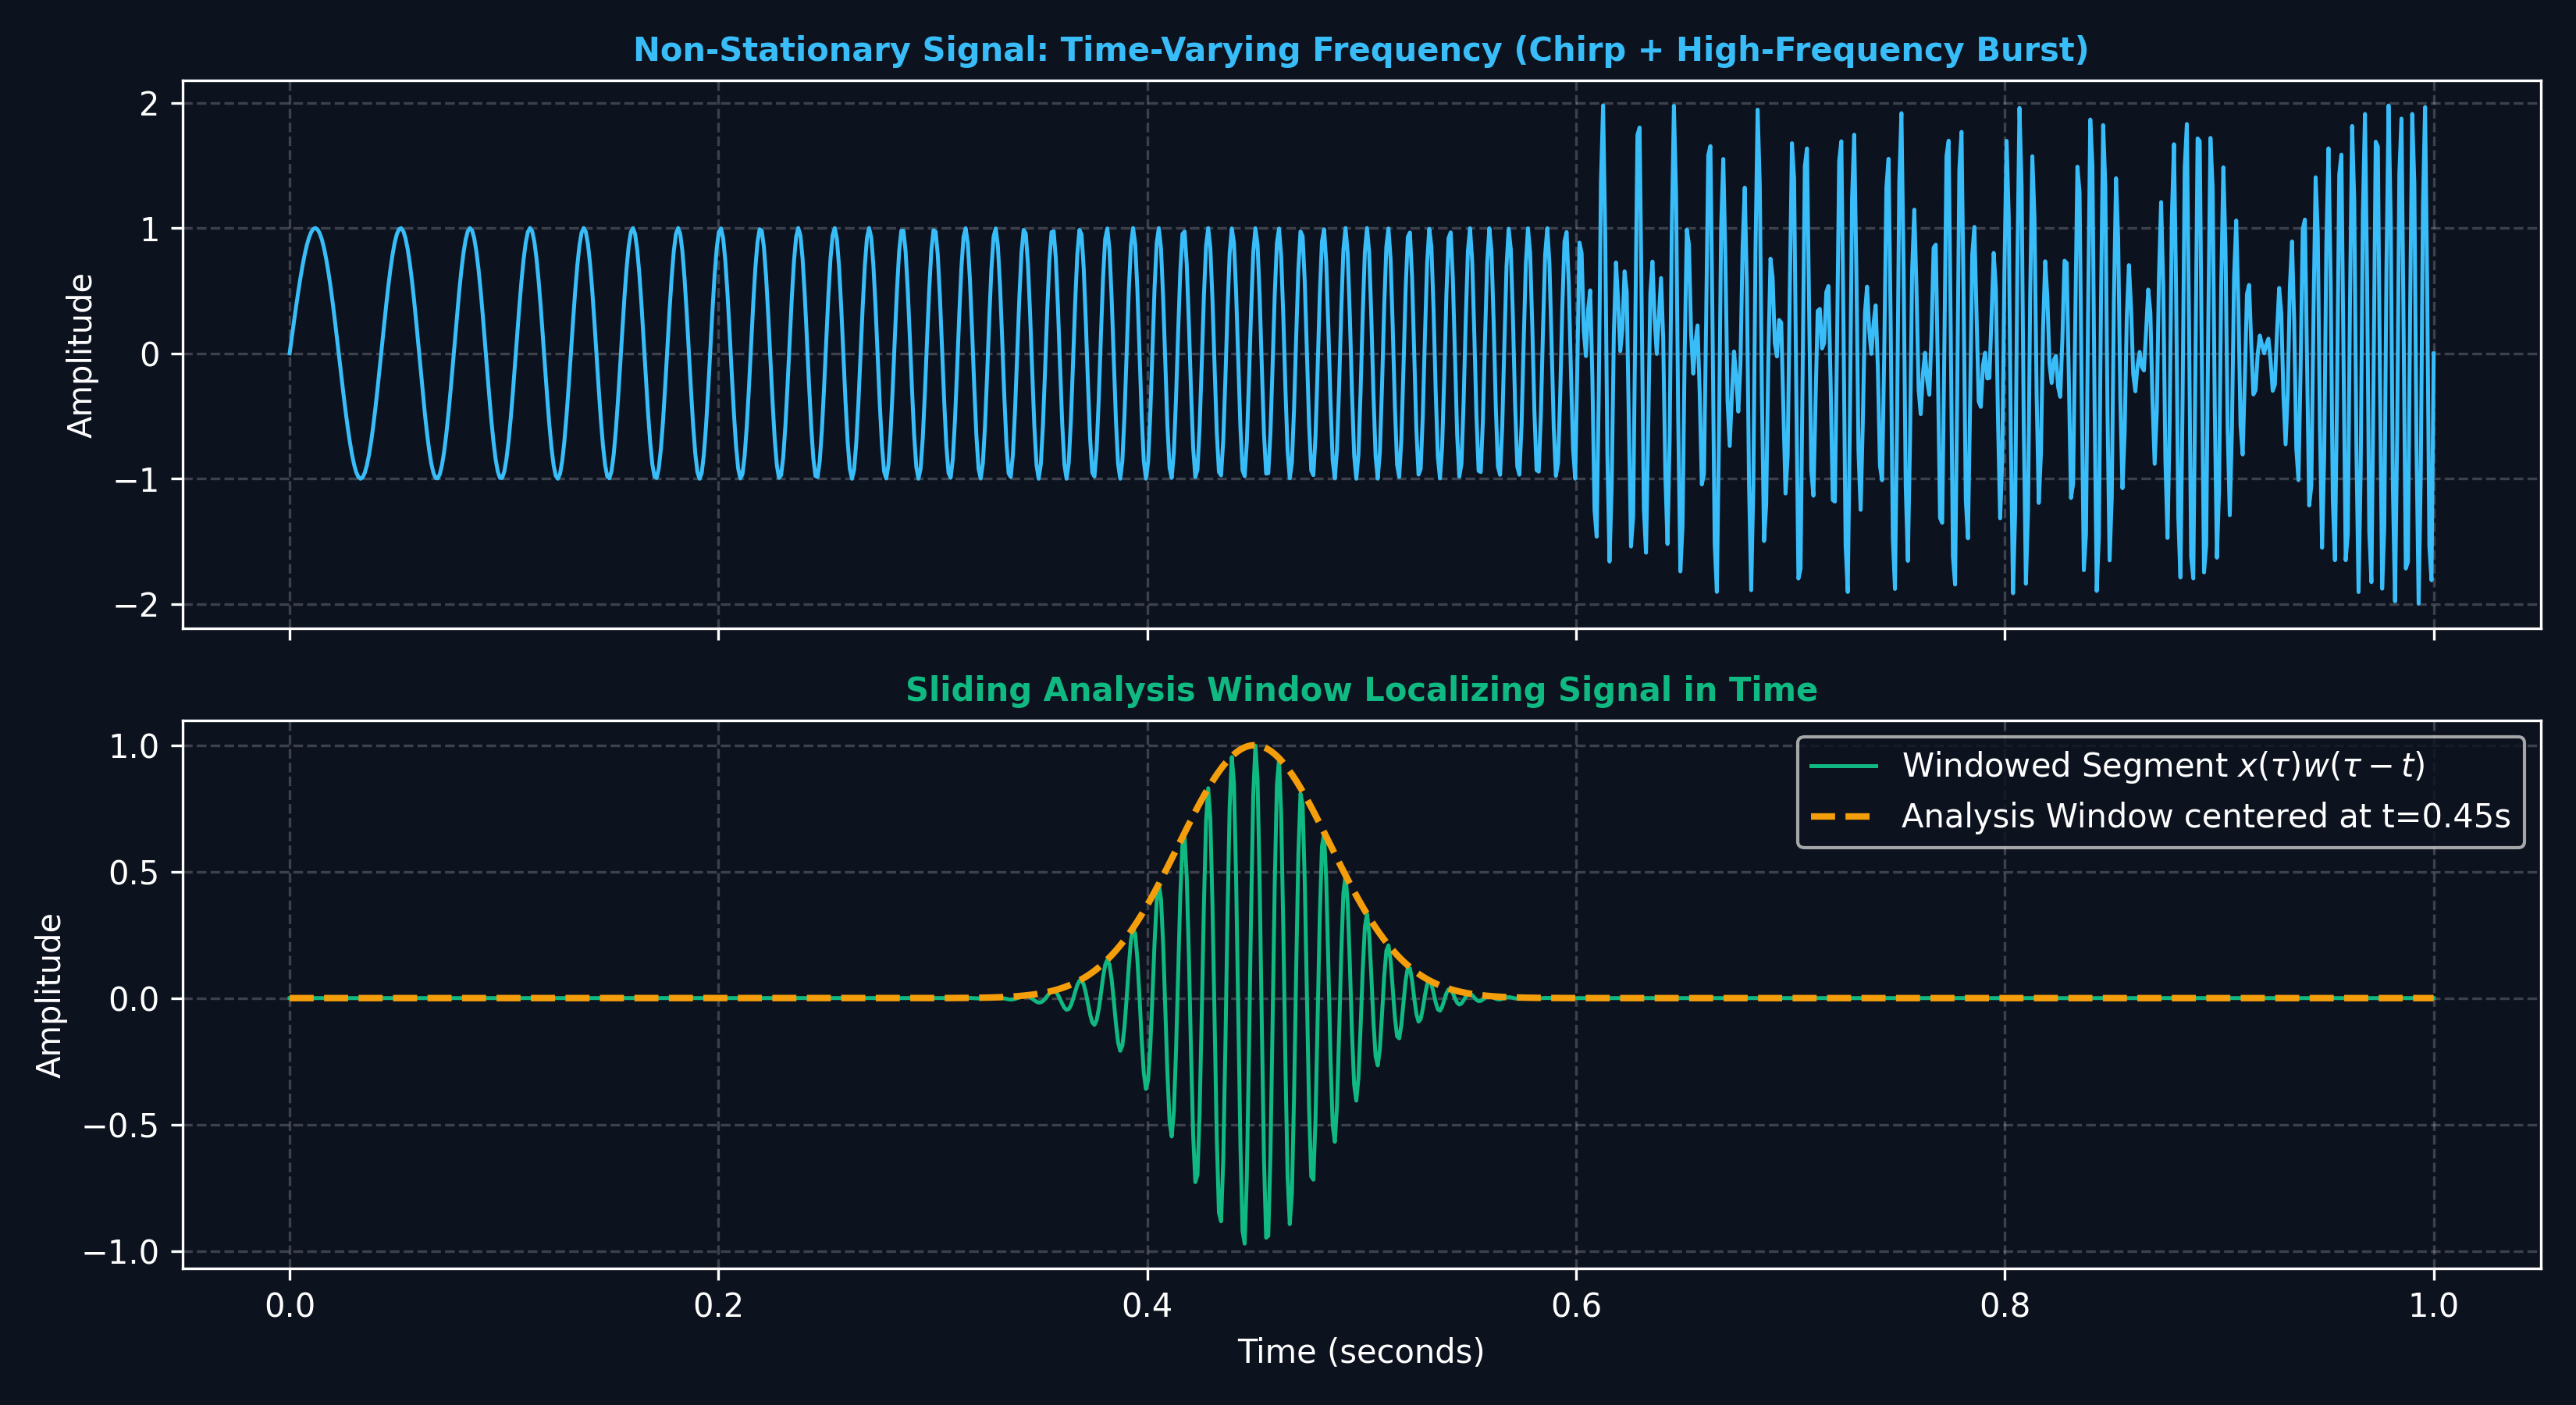
\includegraphics[width=0.85\textwidth]{images/stft_windowing_concept.png}
    \caption{Short-Time Fourier Transform: Sliding Temporal Window Localizing Time-Varying Spectral Content.}
\end{figure}

\begin{figure}[H]
    \centering
    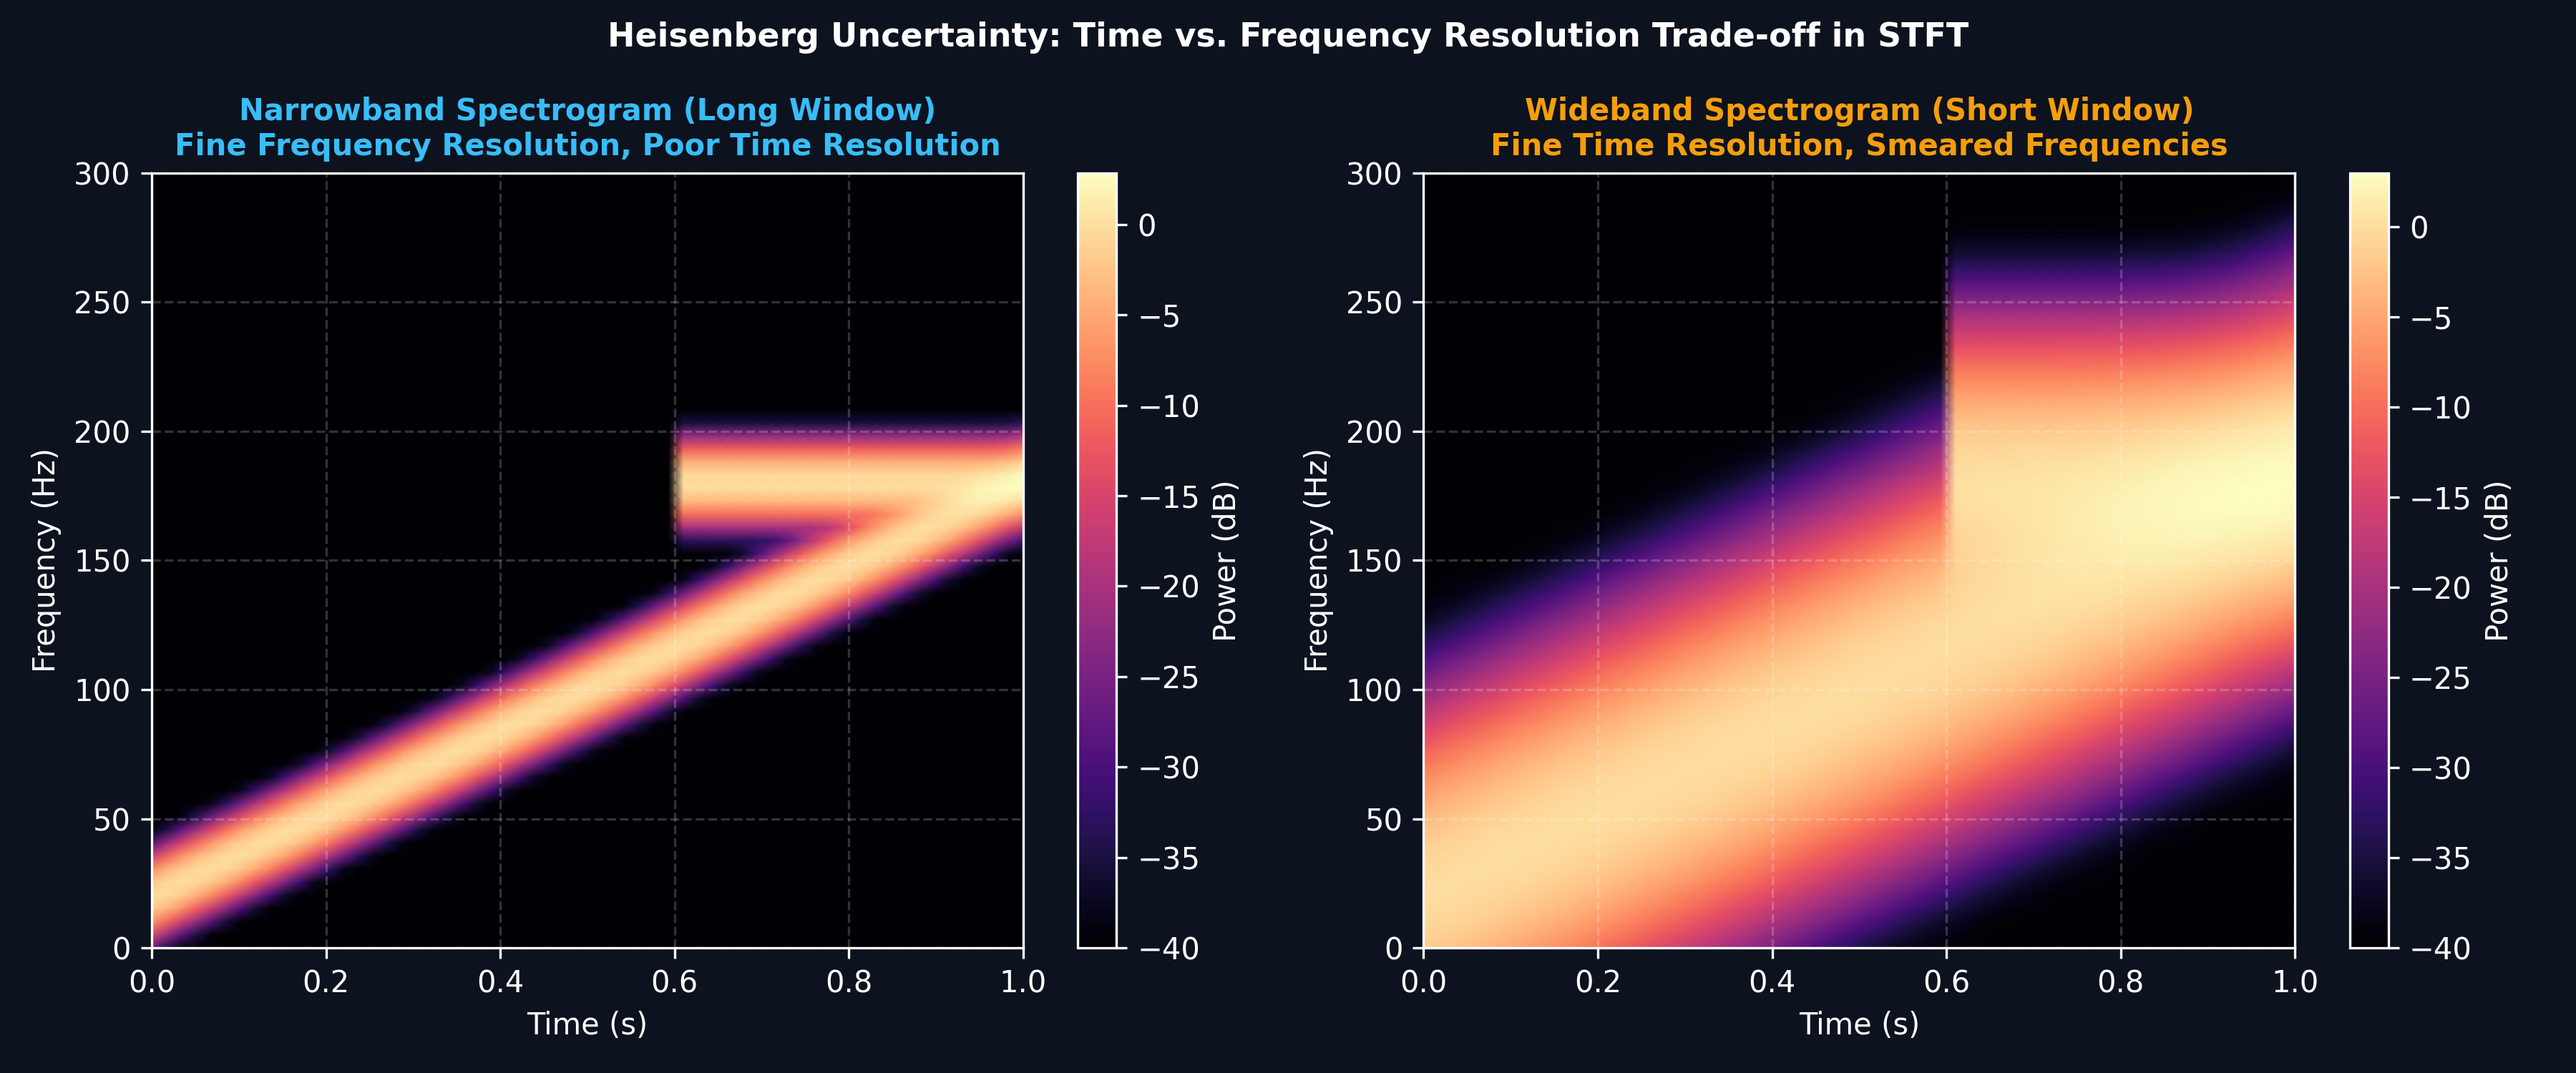
\includegraphics[width=0.85\textwidth]{images/spectrogram_narrowband_vs_wideband.png}
    \caption{Spectrogram Resolution Trade-off: Narrowband (Fine Frequency) vs. Wideband (Fine Time) Representation.}
\end{figure}


To analyze a signal at a specific time $n$, we multiply the signal by a window function $w[m-n]$ centered at time $n$. This window isolates a short segment of the signal around time $n$. We then take the Fourier transform of this isolated segment.

The Short-Time Fourier Transform (STFT) is defined as:
\begin{equation}
X[n, k] = \sum_{m=-\infty}^{\infty} x[m] w[m-n] e^{-j\frac{2\pi}{N}km}
\end{equation}

\textbf{Step-by-Step Breakdown:}
\begin{enumerate}
    \item $x[m]$ is our infinite-length signal.
    \item $w[m-n]$ is the \textbf{analysis window} of length $M$, shifted to time $n$.
    \item $x[m] w[m-n]$ is the windowed signal.
    \item The summation is the $N$-point DFT of the windowed signal.
    \item The result $X[n, k]$ represents the \textbf{local spectrum} of the signal at time $n$.
\end{enumerate}

\section{The Role of the Window Function}
The choice of the window function $w[m]$ is crucial.

\textbf{The Rectangular Window:}
\begin{equation}
w_{rect}[m] = \begin{cases} 1, & 0 \leq m \leq M-1 \\ 0, & \text{otherwise} \end{cases}
\end{equation}
Because the rectangular window has sharp transitions, its frequency response has a narrow mainlobe but very high sidelobes. This causes \textbf{spectral leakage} (Gibbs phenomenon), where energy from one frequency obscures nearby frequencies.

\textbf{Hamming Window:}
To reduce spectral leakage, we taper the window:
\begin{equation}
w_{hamming}[m] = 0.54 - 0.46 \cos\left(\frac{2\pi m}{M-1}\right) \quad \text{for } 0 \leq m \leq M-1
\end{equation}
Tapering reduces sidelobes (less leakage) but widens the mainlobe (decreased frequency resolution).

\section{Time-Frequency Resolution Trade-off}
The \textbf{Heisenberg Uncertainty Principle} states that for continuous signals:
\begin{equation}
\Delta t \cdot \Delta f \geq \frac{1}{4\pi}
\end{equation}
For discrete signals, a similar bound limits the bandwidth-duration product:
\begin{itemize}
    \item \textbf{Wide Window (Large $M$):} Excellent frequency resolution, poor time resolution.
    \item \textbf{Narrow Window (Small $M$):} Excellent time resolution, poor frequency resolution.
\end{itemize}
You cannot simultaneously achieve arbitrarily high resolution in both time and frequency.

\section{Spectrogram}
The \textbf{Spectrogram} visualizes the STFT as a 2D magnitude squared plot:
\begin{equation}
\text{Spectrogram}(n, k) = |X[n, k]|^2
\end{equation}
Practical parameters include window length (e.g., 20-30 ms for speech), hop size (overlap), and FFT size. In a speech spectrogram, vowels appear as dark bands of energy called \textbf{formants}.

\section{Overlap-Add (OLA) Method \& Perfect Reconstruction}
To convert an STFT back to the time domain, we use the Overlap-Add method:
\begin{equation}
x[n] = \frac{\sum_{r=-\infty}^{\infty} y_r[n]}{\sum_{r=-\infty}^{\infty} w[n-rH]}
\end{equation}

\textbf{Theorem:} Perfect reconstruction requires $\sum_r w[n-rH] = C$ (a constant).

\textbf{Proof:}
\begin{enumerate}
    \item Let $y_r[n] = x[n] w[n-rH]$ be the inverse FFT of frame $r$.
    \item Summing these overlapping frames: $\sum_r y_r[n] = \sum_r x[n] w[n-rH] = x[n] \sum_r w[n-rH]$.
    \item If $\sum_r w[n-rH] = C$, then $\sum_r y_r[n] = C x[n] \implies x[n] = \frac{1}{C} \sum_r y_r[n]$.
\end{enumerate}

\section{Alternative Views \& Applications}
\textbf{Wigner-Ville Distribution:} Optimal resolution but introduces artificial cross-terms for multi-component signals.

\textbf{DFT-Bank Interpretation:} STFT can be viewed as passing the signal through a uniform bank of modulated bandpass filters.

\textbf{Applications:} Speech processing (formants), MP3 audio compression (using MDCT), radar Doppler processing, and ECG analysis.

\section{Key Formulas}
\begin{table}[H]
\centering
\begin{tabular}{@{}ll@{}}
\toprule
\textbf{Concept} & \textbf{Formula} \\ \midrule
STFT & $X[n, k] = \sum_{m} x[m] w[m-n] e^{-j\frac{2\pi}{N}km}$ \\
Spectrogram & $S(n, k) = |X[n, k]|^2$ \\
Uncertainty Principle & $\Delta t \cdot \Delta f \geq \frac{1}{4\pi}$ \\
OLA Reconstruction & $x[n] = \frac{\sum_r y_r[n]}{\sum_r w[n-rH]}$ \\ \bottomrule
\end{tabular}
\end{table}

\section{Checkpoint Questions}
\begin{enumerate}
    \item \textbf{Q1:} If you increase the window length $M$, what happens to time and frequency resolution? \\
    \textbf{Answer:} Increasing $M$ spans a longer duration, worsening time resolution but improving frequency resolution (narrower mainlobe).
    \item \textbf{Q2:} Why prefer a Hamming window over rectangular? \\
    \textbf{Answer:} Rectangular windows cause severe spectral leakage due to sharp edges. Hamming windows taper smoothly, reducing sidelobes and leakage.
    \item \textbf{Q3:} What is the maximum hop size $H$ for a rectangular window $w[n]=1$ ($0 \leq n \leq 99$) to satisfy COLA without division? \\
    \textbf{Answer:} $H = 100$. The frames must tile perfectly without gaps or overlapping accumulations to maintain a constant sum of 1.
\end{enumerate}

\end{document}
